\documentclass{standalone}
\usepackage{tikz}
\usepackage{ctex,siunitx}
\usepackage{tkz-euclide}
\usepackage{amsmath}
\usetikzlibrary{patterns, calc}
\usetikzlibrary {decorations.pathmorphing, decorations.pathreplacing, decorations.shapes,}
\begin{document}
\small
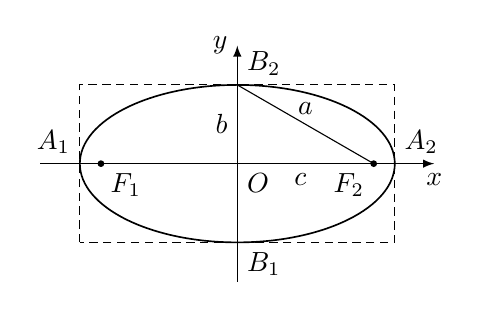
\begin{tikzpicture}[>=latex,scale=1]
  \draw[thin,->](-2.5,0)--(2.5,0)node[below]{$x$};
  \draw[thin,->](0,-1.5)--(0,1.5)node[left]{$y$};
  \draw[semithick](0,0)ellipse(2 and 1);
  \tkzDefPoints{0/0/O,0/-1/B1,0/1/B2}
  \tkzDefPoint({-sqrt(3)},0){F1}
  \tkzDefPoint({sqrt(3)},0){F2}
  \tkzDefPoint(1,{sqrt(3)/2}){M}
  \draw[densely dashed](-2,-1)rectangle(2,1);
  \draw(B2)--(F2)node[midway,above]{$a$};
  \tkzDrawPoints[fill=black](F1,F2)
  \tkzLabelPoint[below right](F1){$F_1$}
  \tkzLabelPoint[below left](F2){$F_2$}
  \tkzLabelPoints[below right](O)
  \node at (-2,0)[above left]{$A_1$};
  \node at (2,0)[above right]{$A_2$};
  \node at (0,-1)[below right]{$B_1$};
  \node at (0,1)[above right]{$B_2$};
  \node at (0,0.5)[left]{$b$};
  \node at (0.8,0)[below]{$c$};
\end{tikzpicture}
\end{document}